\section{Übung - Wiederholung}
\label{sec:uebung_12}

% ##########################################################################
% ############################### Aufgabe 01 ###############################
% ##########################################################################
\label{subsec:uebung_12.aufgabe_01}
\subsection{Aufgabe}
Auf der Instanz GALWAY liegt im (ORACLE-)Directory \textit{STUDENT\_DIR} die CSV Datei \textit{sales4.dat} mit \textit{';'} als Trennzeichen. Auf das Directory \textit{STUDENT\_DIR} wurde ein \textit{'GRANT READ ON DIRECTORY  student\_dir TO PUBLIC'} gemacht.

Der Aufbau dieser CSV Datei:

\begin{table}[H]
  \centering
  \begin{tabular}{|l|l|l|l|l|}
    \hline
    \textbf{Spalte} & \textbf{Datentyp} & \textbf{Bemerkung} \\
    \hline
    PROD\_ID        & integer           & Produktnummer \\
    \hline
    CUST\_ID        & integer           & Customer Nummer \\
    \hline
    TIME\_ID        & DATE              & Verkaufsdatum \\
    \hline
    CHANNEL\_ID     & CHAR(1)           & Vertriebskanal \\
    \hline
    PROMO\_ID       & integer           & aktuelle Werbemaßnahme \\
    \hline
    QUANTITY\_SOLD  & integer           & \multirow{8}{*}{\parbox{7.5cm}{Vierfache Wiederholung einer Gruppierung von Anzahl des verkauften Produktes und des erlösten Betrages}}         \\
    AMOUNT\_SOLD    & number(10,2)      & \\
    QUANTITY\_SOLD1 & integer,          & \\
    AMOUNT\_SOLD1   & number(10,2)      & \\
    QUANTITY\_SOLD2 & integer           & \\
    AMOUNT\_SOLD2   & number(10,2)      & \\
    QUANTITY\_SOLD3 & integer           & \\
    AMOUNT\_SOLD3   & number(10,2)      & \\
    \hline
  \end{tabular}
\end{table}

Die ersten drei Sätze sehen so aus:
\begin{minted}{bash}
  13;987;10-JAN-98;3;999;1;1232.16;11;234.61;25;1935.98;29;1462.95
  13;1660;10-JAN-98;3;999;1;1232.16;44;230.2;67;893.42;84;1564.4
  13;1762;10-JAN-98;3;999;1;1232.16;15;932.14;74;1262.1;11;648.95
\end{minted}


% ############################### Aufgabe 01A ###############################
\subsubsection{Aufgabe}
\label{subsec:uebung_12.aufgabe_01a}
Definieren Sie eine External Table \textit{SALES\_EXTERNAL}.

\paragraph{Lösung}
\label{subsubsec:uebung_12.aufgabe_01a.loesung}
\inputsql{./loesungen/uebung_12/uebung_12_-_aufgabe_01a.sql}


% ############################### Aufgabe 01B ###############################
\subsubsection{Aufgabe}
\label{subsec:uebung_12.aufgabe_01b}
Wie viele verschiedene Kunden haben einen Eintrag in der \textit{sales4.dat} Datei?

\paragraph{Lösung}
\label{subsubsec:uebung_12.aufgabe_01b.loesung}
\inputsql{./loesungen/uebung_12/uebung_12_-_aufgabe_01b.sql}


% ############################### Aufgabe 01C ###############################
\subsubsection{Aufgabe}
\label{subsec:uebung_12.aufgabe_01c}
Wie viele Kunden haben mehr als eine Zeile in der Datei?

\paragraph{Lösung}
\label{subsubsec:uebung_12.aufgabe_01c.loesung}
\inputsql{./loesungen/uebung_12/uebung_12_-_aufgabe_01c.sql}


% ############################### Aufgabe 01D ###############################
\subsubsection{Aufgabe}
\label{subsec:uebung_12.aufgabe_01d}
Welche zwei Produkte haben den geringsten Umsatz erwirtschaftet?

\paragraph{Lösung}
\label{subsubsec:uebung_12.aufgabe_01d.loesung}
\inputsql{./loesungen/uebung_12/uebung_12_-_aufgabe_01d.sql}


% ############################### Aufgabe 01E ###############################
\subsubsection{Aufgabe}
\label{subsec:uebung_12.aufgabe_01e}
Schreiben Sie eine Table Function, die für jeden Kunden, der in der Datei \textit{sales4.dat} enthalten ist, den Gesamtumsatz ermittelt und ausgibt.

\begin{table}[H]
  \centering
  \begin{tabular}{|l|l|l|l|l|}
    \hline
    \textbf{CUST\_ID} & \textbf{GESAMT\_UMSATZ} \\
    \hline
    1660              & 103456,67 \\
    1762              & 5634,90 \\
    \hline
  \end{tabular}
\end{table}

\paragraph{Lösung}
\label{subsubsec:uebung_12.aufgabe_01e.loesung}
\inputsql{./loesungen/uebung_12/uebung_12_-_aufgabe_01e.sql}


% ##########################################################################
% ############################### Aufgabe 02 ###############################
% ##########################################################################
\subsection{Aufgabe}
\label{subsec:uebung_12.aufgabe_02}
Nutzen Sie für die folgende Aufgabe die Tabelle \textit{ORDERS\_JSON} des Schemas \textit{MEURERM}. Geben Sie für jedes Land den insgesamt erwirtschafteten Umsatz je Stadt aus. Zusätzlich soll in einer weiteren Spalte der durchschnittliche Umsatz je Land angezeigt werden.

Aufbau der JSON-Dokumente in \textit{JSON\_CONTENZ}:

\inputjson{./data/uebung_12_-_aufgabe_02.json}

\subsubsection*{Lösung}
\label{subsubsec:uebung_12.aufgabe_02.loesung}
\inputsql{./loesungen/uebung_12/uebung_12_-_aufgabe_02.sql}


% ##########################################################################
% ############################### Aufgabe 03 ###############################
% ##########################################################################
\subsection{Aufgabe}
\label{subsec:uebung_12.aufgabe_03}
Nutzen Sie für die folgenden Aufgaben das DWH-Schema der Instanz GALWAY.

% ############################### Aufgabe 03A ###############################
\subsubsection{Aufgabe}
\label{subsec:uebung_12.aufgabe_03a}
Welche drei Vertriebskanäle waren im Jahr 2010 die Umsatzstärksten?

\paragraph{Lösung}
\label{subsubsec:uebung_12.aufgabe_03a.loesung}
\inputsql{./loesungen/uebung_12/uebung_12_-_aufgabe_03a.sql}

% ############################### Aufgabe 03B ###############################
\subsubsection{Aufgabe}
\label{subsec:uebung_12.aufgabe_03b}
Welche drei Vertriebskanäle waren im Jahr 2010 die Umsatzstärksten?
Geben Sie alle Mitarbeiter aus. Zusätzlich soll das größte Gehalt je Job und Abteilung ausgegeben werden.

\paragraph*{Lösung}
\label{subsubsec:uebung_12.aufgabe_03b.loesung}
\inputsql{./loesungen/uebung_12/uebung_12_-_aufgabe_03b.sql}

% ############################### Aufgabe 03C ###############################
\subsubsection{Aufgabe}
\label{subsec:uebung_12.aufgabe_03c}
Welcher Kunde aus „Middle East and Africa“ hat im Jahr 2014 den größten Umsatz generiert, bezogen auf die Produktkategorie „software“?

\paragraph*{Lösung}
\label{subsubsec:uebung_12.aufgabe_03c.loesung}
\inputsql{./loesungen/uebung_12/uebung_12_-_aufgabe_03c.sql}

% ############################### Aufgabe 03D ###############################
\subsubsection{Aufgabe}
\label{subsec:uebung_12.aufgabe_03d}
Zur Personalübersicht sollen alle Departments mit Anzahl der Mitarbeiter und dem summierten Gehalt ausgegeben werden. Zusätzlich soll diese Information auch noch über alle Departments angezeigt werden.

\paragraph*{Lösung}
\label{subsubsec:uebung_12.aufgabe_03d.loesung}
\inputsql{./loesungen/uebung_12/uebung_12_-_aufgabe_03d.sql}


% ##########################################################################
% ############################### Aufgabe 04 ###############################
% ##########################################################################
\subsection{Aufgabe}
\label{subsec:uebung_12.aufgabe_04}
Erstellen Sie sich lokale Kopien der benötigten Tabellen, sofern Sie keine besitzen. Im Verzeichnis \textit{data} befindet sich die Datei \textit{uebung\_12\_-\_aufgabe\_04.sql} die die unten Abgebildeten SQL-Statements beinhaltet.

\inputsql{./data/uebung_12_-_aufgabe_04.sql}

% ############################### Aufgabe 04A ###############################
\subsubsection{Aufgabe}
\label{subsec:uebung_12.aufgabe_04a}
Erzeugen Sie ein Data Mart basierend auf einem Materialized View, das für jede Region angibt
wie viele Produkte (Menge) über die jeweiligen Absatzkanäle vertrieben wurden.

\paragraph*{Lösung}
\label{subsubsec:uebung_12.aufgabe_04a.loesung}
\inputsql{./loesungen/uebung_12/uebung_12_-_aufgabe_04a.sql}

% ############################### Aufgabe 04B ###############################
\subsubsection{Aufgabe}
\label{subsec:uebung_12.aufgabe_04b}
Erzeugen Sie ein Data Mart basierend auf einem Materialized View, das für jede Region angibt
wie viele Produkte (Menge) über die jeweiligen Absatzkanäle vertrieben wurden.

\paragraph*{Lösung}
\label{subsubsec:uebung_12.aufgabe_04b.loesung}
\inputsql{./loesungen/uebung_12/uebung_12_-_aufgabe_04b.sql}


% ##########################################################################
% ############################### Aufgabe 05 ###############################
% ##########################################################################
\label{subsec:uebung_12.aufgabe_05}
\subsection{Aufgabe}
\begin{itemize}
  \item Zeige für jede Bestellung an, wie hoch der Bestellwert der Vorgänger-Bestellung war.
  \item Ermittle zusätzlich für jede Bestellung den durchschnittlichen Bestellwert für die aktuelle Bestellung, den direkten zeitlichen Nachfolger und Vorgänger.
\end{itemize}

\begin{figure}[H]
  \centering
  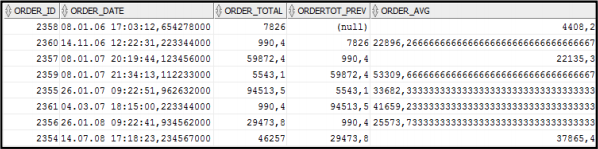
\includegraphics[width=1\textwidth]{img//uebung_12_-_aufgabe_05.png}
  \label{img:uebung_12_-_aufgabe_05}
\end{figure}

\subsubsection{Lösung}
\label{subsubsec:uebung_12.aufgabe_05.loesung}
\inputsql{./loesungen/uebung_12/uebung_12_-_aufgabe_05.sql}


% ##########################################################################
% ############################### Aufgabe 06 ###############################
% ##########################################################################
\subsection{Aufgabe}
\label{subsec:uebung_12.aufgabe_06}
Zeige für jeden Mitarbeiter das höchste Gehalt in seiner Abteilung und innerhalb seines Jobs.

\begin{figure}[H]
  \centering
  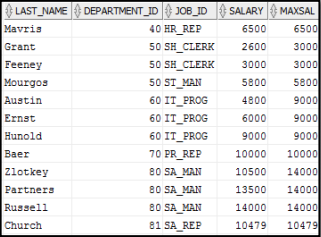
\includegraphics[width=0.55\textwidth]{img//uebung_12_-_aufgabe_06.png}
  \label{img:uebung_12_-_aufgabe_06}
\end{figure}

\subsubsection*{Lösung}
\label{subsubsec:uebung_12.aufgabe_06.loesung}
\inputsql{./loesungen/uebung_12/uebung_12_-_aufgabe_06.sql}


% ##########################################################################
% ############################### Aufgabe 07 ###############################
% ##########################################################################
\subsection{Aufgabe}
\label{subsec:uebung_12.aufgabe_07}
Zeige für jede Bestellung den in dem betreffenden Jahr insgesamt erwirtschafteten Umsatz (Summe aller Bestellwerte).

\begin{figure}[H]
  \centering
  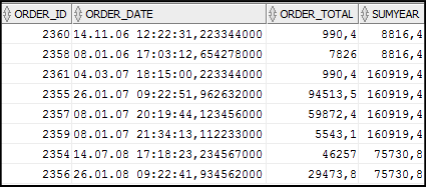
\includegraphics[width=0.75\textwidth]{img//uebung_12_-_aufgabe_07.png}
  \label{img:uebung_12_-_aufgabe_07}
\end{figure}

\subsubsection*{Lösung}
\label{subsubsec:uebung_12.aufgabe_07.loesung}
\inputsql{./loesungen/uebung_12/uebung_12_-_aufgabe_07.sql}


% ##########################################################################
% ############################### Aufgabe 08 ###############################
% ##########################################################################
\subsection{Aufgabe}
\label{subsec:uebung_12.aufgabe_08}
Welche 2 Mitarbeiter haben die meisten Bestellungen bearbeitet (SALES\_REP\_ID in ORDERS)?

\subsubsection*{Lösung}
\label{subsubsec:uebung_12.aufgabe_08.loesung}
\inputsql{./loesungen/uebung_12/uebung_12_-_aufgabe_08.sql}


% ##########################################################################
% ############################### Aufgabe 09 ###############################
% ##########################################################################
\subsection{Aufgabe}
\label{subsec:uebung_12.aufgabe_09}

% ############################### Aufgabe 09a ###############################
\subsubsection{Aufgabe}
\label{subsec:uebung_12.aufgabe_09a}
Gebt für jede Produktoberkategorie die Umsätze der Jahre 2014 bis 2016 in einer Zeile an. Die Umsätze der einzelnen Jahre sollen dabei in einer separaten Spalte dargestellt werden.

\begin{figure}[H]
  \centering
  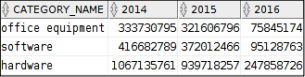
\includegraphics[width=0.50\textwidth]{img//uebung_12_-_aufgabe_09a.png}
  \label{img:uebung_12_-_aufgabe_09a}
\end{figure}

\paragraph*{Lösung}
\label{subsubsec:uebung_12.aufgabe_09a.loesung}
\inputsql{./loesungen/uebung_12/uebung_12_-_aufgabe_09a.sql}

% ############################### Aufgabe 09b ###############################
\subsubsection{Aufgabe}
\label{subsec:uebung_12.aufgabe_09b}
Nutzt den Pivot Operator um die Abfrage aus a) abzubilden.

\paragraph*{Lösung}
\label{subsubsec:uebung_12.aufgabe_09b.loesung}
\inputsql{./loesungen/uebung_12/uebung_12_-_aufgabe_09b.sql}


% ##########################################################################
% ############################### Aufgabe 10 ###############################
% ##########################################################################
\subsection{Aufgabe}
\label{subsec:uebung_12.aufgabe_10}

% ############################### Aufgabe 10a ###############################
\subsubsection{Aufgabe}
\label{subsubsec:uebung_12.aufgabe_10a}
Schreibe eine Table Function die zu jedem Mitarbeiter die Anzahl der bearbeiteten Bestellungen, den größten Bestellumsatz, seine Abteilung und die Anzahl der Mitarbeiter, die in derselben Abteilung arbeiten, ausgibt.

\begin{table}[H]
  \centering
  \small
  \fontfamily{courier_new}
  \begin{tabular}{|l|l|l|l|l|l|l|}
    \hline
    EMPNO        & EMP               & C*\_O & MAX\_SALES & DEPNO & DEPT             & C*\_ED \\
    \hline
     200         & Jennifer Whalen   & 0     &            & 10    & Administration   & 1 \\
     202         & Pat Fay           & 0     &            & 20    & Marketing        & 2 \\
     201         & Michael Hartstein & 0     &            & 20    & Marketing        & 2 \\
     117         & Sigal Tobias      & 0     &            & 30    & Purchasing       & 2 \\
     203         & Susan Mavris      & 0     &            & 40    & Human Resources  & 1 \\
     197         & Kevin Feeney      & 0     &            & 50    & Shipping         & 3 \\
     199         & Douglas Grant     & 0     &            & 50    & Shipping         & 3 \\
     104         & Bruce Ernst       & 0     &            & 60    & IT               & 3 \\
     105         & David Austin      & 0     &            & 60    & IT               & 3 \\
     204         & Hermann Baer      & 0     &            & 70    & Public Relations & 1 \\
     145         & John Russell      & 1     & 46257      & 80    & Sales Europe     & 3 \\
     $[$\dots$]$ &                   &       &            &       &                  & \\
     \hline
  \end{tabular}
\end{table}

\paragraph*{Lösung}
\label{subsubsec:uebung_12.aufgabe_10a.loesung}
\inputsql{./loesungen/uebung_12/uebung_12_-_aufgabe_10a.sql}

% ############################### Aufgabe 10b ###############################
\subsubsection{Aufgabe}
\label{subsec:uebung_12.aufgabe_10b}
Ändere die Table Function aus Aufgabe \ref{subsubsec:uebung_12.aufgabe_10a} in eine Pipelined Table Function.

\paragraph*{Lösung}
\label{subsubsec:uebung_12.aufgabe_10b.loesung}
\inputsql{./loesungen/uebung_12/uebung_12_-_aufgabe_10b.sql}


% ##########################################################################
% ############################### Aufgabe 11 ###############################
% ##########################################################################
\subsection{Aufgabe}
\label{subsec:uebung_12.aufgabe_11}
Schreibe eine Procedure die mittels Native Dynamic SQL alle Kundennamen ausgibt die einem übergebenen Pattern entsprechen. Dabei soll Groß- bzw. Kleinschreibung nicht berücksichtigt 
werden.

\begin{minted}[linenos, autogobble, breaklines,]{sql}
  EXEC p_dynsql('%cl%');
  Clint Chapman
  Clint Gielgud
  Cliff Puri
  PL/SQL-Prozedur erfolgreich abgeschlossen.
\end{minted}

\subsubsection*{Lösung}
\label{subsubsec:uebung_12.aufgabe_11.loesung}
\inputsql{./loesungen/uebung_12/uebung_12_-_aufgabe_11.sql}


% ##########################################################################
% ############################### Aufgabe 12 ###############################
% ##########################################################################
\subsection{Aufgabe}
\label{subsec:uebung_12.aufgabe_12}
Welche Mitarbeiter haben mindestens 2-mal den Job gewechselt? Gebe zusätzlich die Anzahl der vorherigen Jobs, den aktuellen Job sowie das Startdatum des aktuellen Jobs an.

\begin{figure}[H]
  \centering
  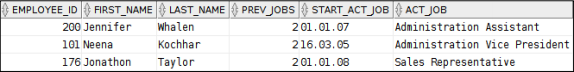
\includegraphics[width=1\textwidth]{img//uebung_12_-_aufgabe_12.png}
  \label{img:uebung_12_-_aufgabe_12}
\end{figure}

\subsubsection*{Lösung}
\label{subsubsec:uebung_12.aufgabe_12.loesung}
\inputsql{./loesungen/uebung_12/uebung_12_-_aufgabe_12.sql}


% ##########################################################################
% ############################### Aufgabe 13 ###############################
% ##########################################################################
\subsection{Aufgabe}
\label{subsec:uebung_12.aufgabe_13}
Ermittelt für alle Monate im Jahr 2010 die Umsätze in der Produkt Category ‚Software‘ in diesem Monat und klassifiziere diese in ‘klein‘, ‘mittel‘ und ‘gross‘.Die Ausgabe könnte wie folgt aussehen:

\begin{table}[H]
  \begin{tabular}{|l|l|l|l|l|l|l|}
    \hline
    \textbf{MONTH}   & \textbf{SALES}   & \textbf{CATEGORY} \\
    \hline
    2010-01 & 1139699 & mittel \\
    2010-02 & 1521220 & gross \\
    2010-03 & 1067636 & klein \\
    2010-04 & 1550019 & gross \\
    2010-05 & 1010877 & klein \\
    2010-06 & 1071852 & klein \\
    2010-07 & 1509785 & gross \\
    2010-08 & 1287540 & mittel \\
    2010-09 & 2325681 & gross \\
    2010-10 & 1415155 & mittel \\
    2010-11 & 1210609 & mittel \\
    2010-12 & 850281  & klein \\
     \hline
  \end{tabular}
\end{table}

\subsubsection*{Lösung}
\label{subsubsec:uebung_12.aufgabe_13.loesung}
\inputsql{./loesungen/uebung_12/uebung_12_-_aufgabe_13.sql}


% ##########################################################################
% ############################### Aufgabe 14 ###############################
% ##########################################################################
\subsection{Aufgabe}
\label{subsec:uebung_12.aufgabe_14}

% ############################### Aufgabe 14a ###############################
\subsubsection{Aufgabe}
\label{subsubsec:uebung_12.aufgabe_14a}
Schreibe eine Table Function, der eine Referenz auf einen Cursor übergeben wird. Dieser soll Bestelldatensätze beinhalten und es soll für jede übergebene Bestellung die \textit{order\_id}, das \textit{Bestelldatum}, die \textit{Anzahl der Bestellpositionen}, der \textit{Absatzkanal} und der \textit{Name des Kunden} ausgegeben werden.

Ein Aufruf der Funktion könnte wie folgt aussehen:
\begin{minted}[linenos, autogobble, breaklines,]{sql}
SELECT * 
FROM TABLE(
  tf_prod(CURSOR(SELECT * FROM orders WHERE order_id <2356))
);
\end{minted}

\paragraph*{Lösung}
\label{subsubsec:uebung_12.aufgabe_14a.loesung}
\inputsql{./loesungen/uebung_12/uebung_12_-_aufgabe_14a.sql}

% ############################### Aufgabe 14b ###############################
\subsubsection{Aufgabe}
\label{subsec:uebung_12.aufgabe_14b}
Ändere die Table Function aus Aufgabe \ref{subsubsec:uebung_12.aufgabe_14a} in eine Pipelined Table Function.

\paragraph*{Lösung}
\label{subsubsec:uebung_12.aufgabe_14b.loesung}
\inputsql{./loesungen/uebung_12/uebung_12_-_aufgabe_14b.sql}


% ##########################################################################
% ############################### Aufgabe 15 ###############################
% ##########################################################################
\subsection{Aufgabe}
\label{subsec:uebung_12.aufgabe_15}
Zeigen Sie, wie im abgebildeten Schema eine Änderung des Attributes \glqq{}LastName\grqq{} der Tabelle \glqq{}DimSalesPerson\grqq{} nach 

\begin{itemize}[itemsep=0pt]
  \item[a)] Typ 2
  \item[b)] Typ 4
\end{itemize}

aussehen würde.


\begin{figure}[H]
  \centering
  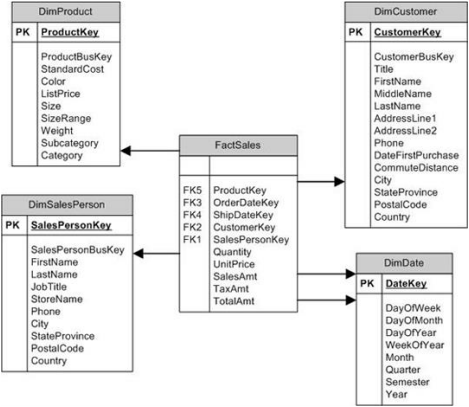
\includegraphics[width=0.75\textwidth]{img//uebung_12_-_aufgabe_15.png}
  \label{img:uebung_12_-_aufgabe_15}
  \caption{Schema}
\end{figure}
